\documentclass[12pt,a4paper,article,english,firamath]{nsi}
\pagestyle{empty}
\begin{document}
\titre{A chessboard and dominoes}
\classe{Euro 1\ere}
\maketitle
Assemble by teams of 2 and try to find the answers to the following problems.\\ For each problem solved, you get 3 points !

\subsection*{Problem 1}

Is it possible to cover a whole chessboard with non-overlapping dominoes ? 

\subsection*{Problem 2}

One corner has been removed from a chessboard. Is it possible to cover the remaining portion of the board with dominoes so that each domino covers exactly two squares?\\
What if two opposite corners are removed ?

\subsection*{Problem 3}

Two arbitrary but adjacent squares have been removed from a chessboard. Is it possible to cover the rectangleemaining portion of the board with dominoes?

\subsection*{Problem 4}

Two arbitrary squares of different colors have been removed from a chessboard. Is it possible to cover the remaining portion of the board with dominoes?

\subsection*{Problem 5}

Two arbitrary pairs of squares of different colors have been removed from a chessboard. Is it always possible to cover the remaining portion of the board with dominoes?

\subsection*{Problem 6}

Three arbitrary pairs of squares of different colors have been removed from a chessboard, so that the chessboard does not split into two or more separate pieces. Is it always possible to cover the remaining portion of the board with
dominoes?

\subsection*{Problem 7}

A domino has two edges, a long edge and a short edge. Two adjacent dominoes must be in one of the only three possible
configurations : long edge to long edge, short edge to short edge and long edge to short edge.\\ In a domino tiling of a
chessboard, what is the minimum number of long-edge to long-edge pairs ?

\subsection*{Problem 8}

Prove that in any cover of a whole chessboard with dominoes, the number of horizontal
dominoes with a black left square and the number of horizontal dominoes with a white left square are equal.

\begin{center}
\titlefont\LARGE\color{UGLiBlue} Chessboard\\[2em]


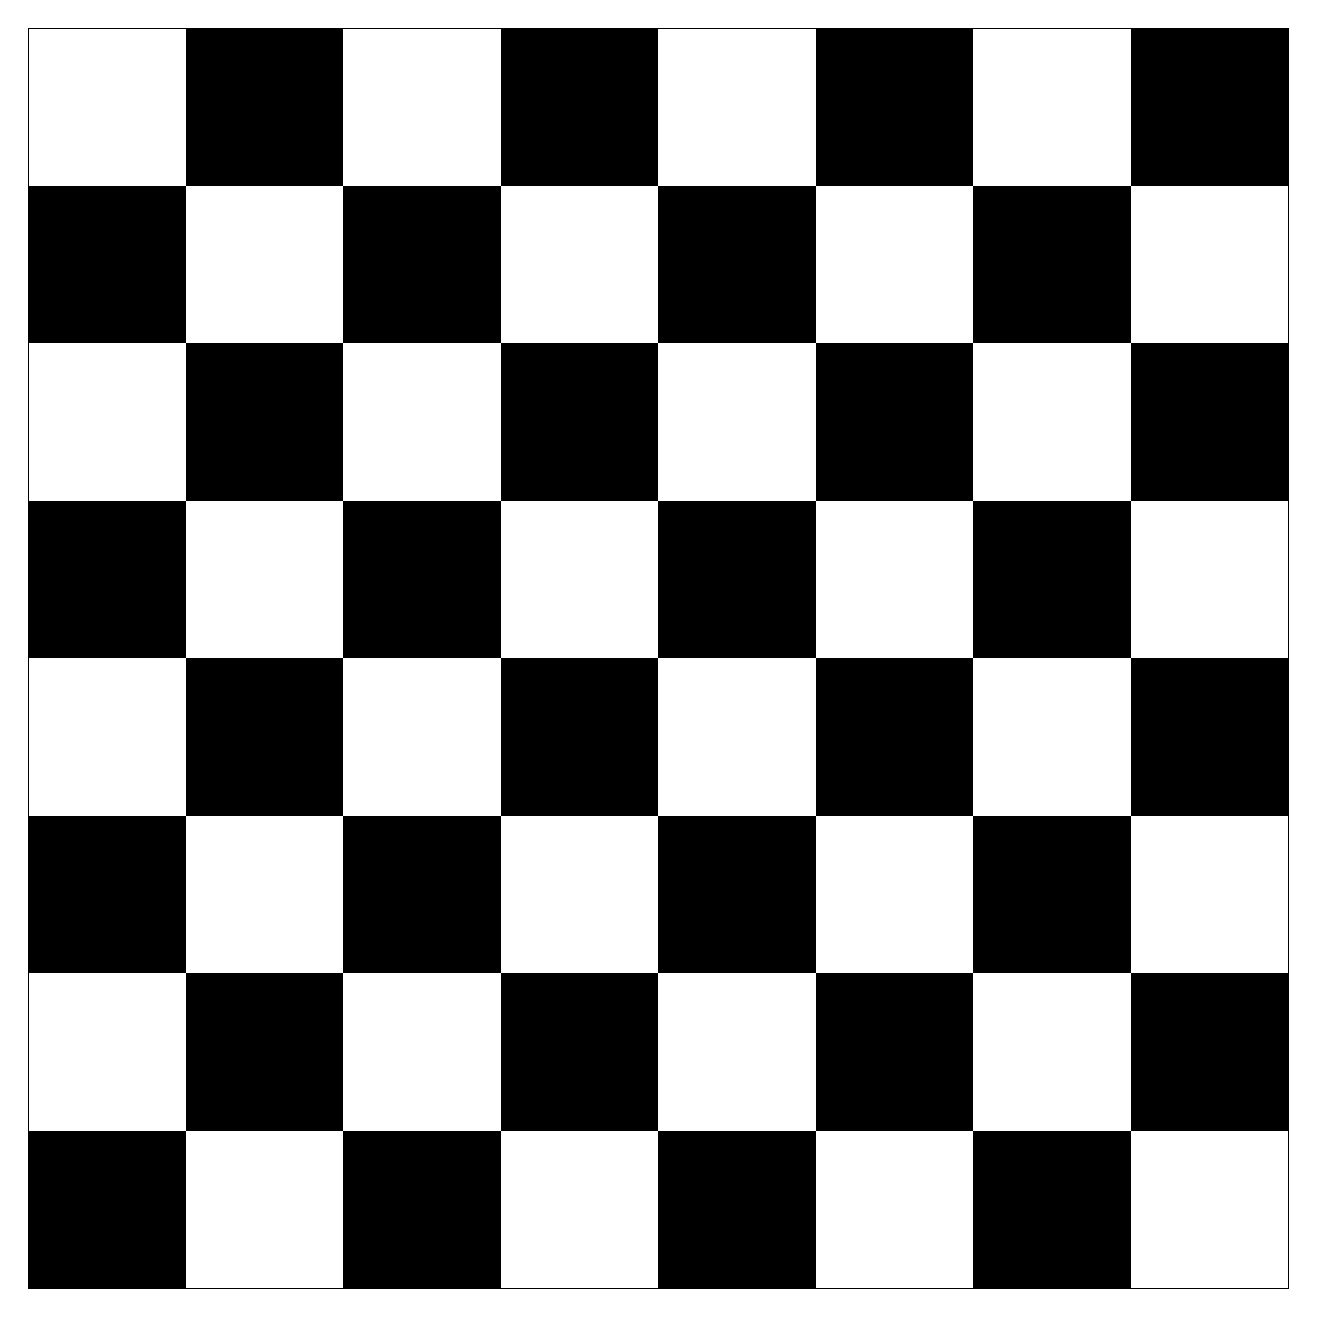
\begin{tikzpicture}[scale=2]
    \foreach \i in {0,1,...,7} {
      \foreach \j in {0,1,...,7} {
        \pgfmathtruncatemacro{\shade}{mod(\i+\j,2)}
        \ifnum\shade=0
          \fill[black] (\i,\j) rectangle ++(1,1);
        \else
          \fill[white] (\i,\j) rectangle ++(1,1);
        \fi
      }
    }
    \draw (0,0) rectangle (8,8);
  \end{tikzpicture}


\newpage
Dominoes\\[2em]

\begin{tikzpicture}[scale=2]
  \foreach \i in {0,1,...,7} {
    \foreach \j in {0,2,...,6} {
    \pgfmathtruncatemacro{\shade}{mod(\i+\j,3)}
    \ifnum\shade=0
      \draw[fill=UGLiBlue!50] (\i,\j) rectangle ++(1,2);
    \else
    \ifnum\shade=1
    \draw[fill=UGLiRed!50] (\i,\j) rectangle ++(1,2);
    \else
    \draw[fill=UGLiGreen!50] (\i,\j) rectangle ++(1,2);
    \fi
    \fi
    }
    }
\end{tikzpicture}
\end{center}
\end{document}